% QTML 2026 extended abstract (non-archival, non-anonymous).
% Submit as a contributed talk: up to 3 pages excluding references. This compiles to ~2 pages
% including the figure, which is within the talk limit (it would exceed the 1-page poster limit).
\documentclass[11pt]{article}
\usepackage[letterpaper,margin=1in]{geometry}
\usepackage[T1]{fontenc}
\usepackage{amsmath,amssymb}
\usepackage{graphicx}
\usepackage[hidelinks]{hyperref}
\graphicspath{{../figures/}}
\pagestyle{empty}
\setlength{\parskip}{4pt}

\begin{document}
\begin{center}
{\Large\bfseries \textsc{SimCert}: A Classical-Simulability Audit of Trained Quantum-NLP Text Classifiers}\\[6pt]
{\normalsize Tanvir Ahmed$^{1}$}\\[2pt]
{\small $^{1}$North South University, Dhaka, Bangladesh \quad\textbullet\quad tanvir.ahmed32@northsouth.edu}\\[2pt]
{\small Submission type: contributed talk / poster \quad\textbullet\quad Track: Quantum NLP; Benchmarking and Complexity}
\end{center}
\vspace{2pt}

Quantum natural language processing (QNLP) models, from compositional DisCoCat circuits to
quantum self-attention networks and all-quantum token mixers, are promoted for a quantum benefit
on text classification. That benefit is usually argued from accuracy, yet whether a \emph{trained}
QNLP circuit ever leaves the efficiently classically-simulable regime is rarely tested. The same
question was recently settled for tabular quantum machine learning and for quantum convolutional
networks, and the theory that trainable variational models are constrained matrix product states
(MPS) makes it concrete for language too. We ask which published QNLP results survive a classical
surrogate of the trained circuit.

We introduce \textsc{SimCert}, an open and model-agnostic protocol. It re-simulates each trained
circuit as a bond-dimension-$\chi$ MPS, sweeps $\chi$, and records the smallest value $\chi^\star$
at which a classical surrogate recovers the model's own predictions, together with an
entanglement-removal ablation, the state entanglement entropy, a geometric-difference kernel test,
and a data-reuploading spectral test. A single audit consumer treats every model uniformly through
a common circuit representation, including a mixed-state purification path for models whose readout
is a reduced density matrix.

We audit five published architectures, namely DisCoCat as realised in lambeq, the quantum
self-attention models QSANN and QMSAN, the all-quantum token mixer CLAQS, and a variational
reference classifier, across four datasets and up to ten qubits. A classical surrogate recovers the
predictions at small and non-growing bond dimension. Attention and mixer models are recovered at
$\chi{=}1$, that is by a product state, and the compositional model at $\chi{=}2$. As we grow the
qubit count on a fixed task, $\chi^\star$ stays flat while the exact-MPS bound $2^{n/2}$ grows
exponentially (Figure~\ref{fig:qtml}). The trained circuits carry entanglement, with mean bipartite
entropy from about $0.1$ to $1.3$ nats, but removing it barely moves the result, so the entanglement
is present without being load-bearing for the decision. The one revealing exception is the
compositional model, whose grammar cups make $\chi{=}1$ collapse toward chance, which is why it alone
needs $\chi{=}2$.

We read this cautiously. It suggests that the quantum resource is not the operative ingredient at
the scales these models are tested, not that QNLP is classically simulable in general. We release
the harness and phrase the finding as a protocol and a set of questions for QNLP model and benchmark
design, chief among them which architectural choices, if any, make $\chi^\star$ grow with system
size. A full write-up and the open-source harness accompany this abstract.

\begin{figure}[h]
\centering
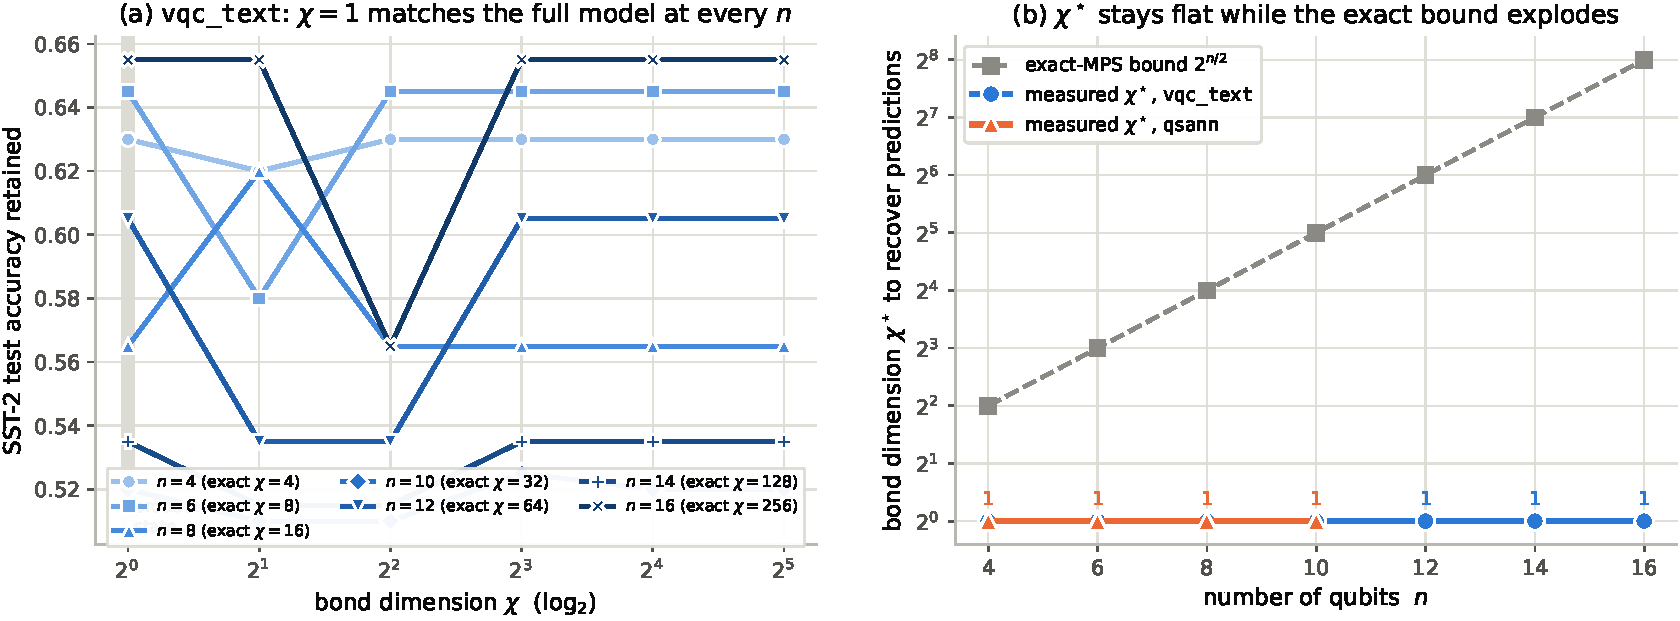
\includegraphics[width=0.92\linewidth]{scaling.pdf}
\caption{\small $\chi^\star$ stays flat at $1$ as the reference model grows from four to ten qubits
(right, orange), while the exact-MPS bound $2^{n/2}$ grows exponentially (grey). Left, accuracy is
flat in $\chi$ at every size, so a product-state surrogate recovers the predictions throughout.}
\label{fig:qtml}
\end{figure}

\end{document}
